\section{Synchronization Channels}
\label{sec:modeling:channels}
\begin{figure}[hbt!]
\begin{center}
\begin{tikzpicture}[
  font=\sffamily,
  every matrix/.style={ampersand replacement=\&,column sep=2cm,row sep=2cm},
  source/.style={draw,thick,rounded corners,fill=yellow!20,inner sep=.3cm},
  process/.style={draw,thick,circle,fill=blue!20},
  sink/.style={source,fill=green!20},
  datastore/.style={draw,very thick,shape=datastore,inner sep=.3cm},
  dots/.style={gray,scale=2},
  to/.style={->,>=stealth',shorten >=1pt,semithick,font=\sffamily\footnotesize},
  every node/.style={align=center}]

  % Position the nodes using a matrix layout
  \matrix{
    \node[source] (core0) {Core 0};
      \& \node[source] (cache0) {Cache 0};
      \\

    \node[source] (queryfifo0) {Query FIFO 0}; \& \&
    \node[source] (datafifo0) {Data FIFO 0};
    \\
      \& \node[sink] (databus) {Data Bus}; \&
      \\
      \node[sink] (querybus) {Query Bus}; \&
      \node[sink] (queryfifomgr) {Query FIFO Mgr};\&
      \node[sink] (datafifomem) {Data FIFO Mem};
      \\\\
      \& \node[sink] (cmgr) {Coherence Manager}; \&
      \node[sink] (mem) {Memory};\\
  };

  % Draw the arrows between the nodes and label them.
  \draw[to] (core0) to[bend left=5] node[midway,above] {$CPU\_REQ[0]$} (cache0);
  \draw[to] (cache0) to[bend left=5] node[midway,below] {$CPU\_ACK[0]$} (core0);

  \draw[to] (queryfifo0) to[bend left=5] node[midway,above,sloped] {\!\!\!\!\!\!\!\!$QUERY\_IN[0]$} (cache0);
  \draw[to] (cache0) to[bend left=5] node[midway,below,sloped] {$QUERY\_OUT[0]$} (queryfifo0);
  \draw[to] (datafifo0) to[bend left=5] node[midway,below,sloped] {$DATA\_IN[0]$} (cache0);
  \draw[to] (cache0) to[bend left=5] node[midway,above,sloped] {$DATA\_OUT[0]$} (datafifo0);
%  \draw[to] (daq) -- node[midway,right] {raw event data\\level 1} (buffer);
  \draw[to] (queryfifo0) to[bend left=5] node[midway,above,sloped] {$QUERY\_TO\_BUS[0]$} (querybus);
  \draw[to] (querybus) to[bend left=5] node[midway,above,sloped] {$QUERY\_BROADCAST$} (queryfifo0);


  \draw[to] (datafifo0) to[bend left=5] node[midway,below,sloped] {$DATA\_TO\_BUS$} (databus);
  \draw[to] (databus) to[bend left=5] node[midway,above,sloped] {$DATA\_TRANS[0]$} (datafifo0);
  \draw[to] (datafifomem) to[bend left=5] node[midway,below,sloped] {$DATA\_TO\_BUS$} (databus);
  \draw[to] (databus) to[bend left=5] node[midway,above,sloped] {$DATA\_TRANS[MEM\_ID]$} (datafifomem);

  \draw[to] (cmgr) to[bend left=5] node[midway,above,sloped] {$MEM\_READ$} (mem);
  \draw[to] (cmgr) to[bend right=5] node[midway,below,sloped] {$MEM\_WRITE$} (mem);
  \draw[to] (datafifomem) to[bend right=5] node[midway,above,sloped] {$DATA\_IN[MEM\_ID]$} (cmgr);
  \draw[to] (cmgr) to[bend right=5] node[midway,below,sloped] {$DATA\_OUT[MEM\_ID]$} (datafifomem);

  \draw[to] (querybus) to[bend left=15] node[midway,above,sloped]
  {$QUERY\_BROADCAST$} (queryfifomgr);

  \draw[to] (queryfifomgr) to[bend right=5] node[midway,below,sloped]
  {$QUERY\_IN[MGR\_IN]$} (cmgr);

  \draw[to] (mem) to[bend right=5] node[midway,above,sloped] {$DATA\_OUT[MEM\_ID]$} (datafifomem);
\end{tikzpicture}

\end{center}
\caption{Recurring Synchronizations in the Model}
\label{fig:UPPAAL:Comms}
\end{figure}
Figure~\ref{fig:UPPAAL:Comms} shows how synchronizations between the
automata are organized. Some synchronizations, only intended to ensure the
proper function of the model, are omitted from the figure, namely
\textbf{SYS\_INIT}, which initializes each automaton, \textbf{FORCE\_URGENT}
and \textbf{FORCE\_EXTRA\_URGENT}, which are used to make a transition
\textit{urgent} and increase its \textit{priority}. These last two
synchronizations are performed using the automaton shown in
Figure~\ref{fig:UPPAAL:ForceUrgent}.

\begin{figure}[hbt!]
\begin{center}
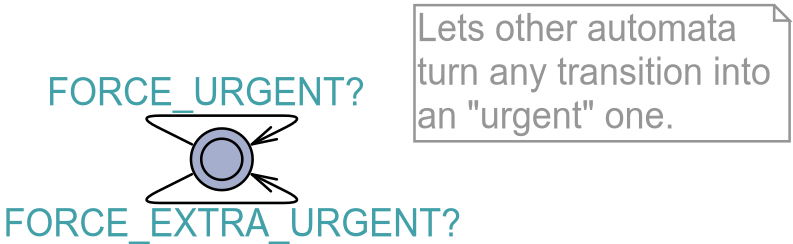
\includegraphics[width=0.4\textwidth]{\chapterdirectory/figure/ForceUrgent.pdf}
\end{center}
\caption{Purely Utilitarian Automaton}
\label{fig:UPPAAL:ForceUrgent}
\end{figure}

The synchronization channels shown in the figure can be categorized as follows.

\paragraph{Query Transfer:}
\begin{itemize}
\item \textbf{QUERY\_BROADCAST:}
   \texttt{urgent}, \texttt{broadcast} channel used to synchronize with
   automata waiting for an incoming query.

\item \textbf{QUERY\_TO\_BUS:}
   \texttt{urgent} channel used to send a query to the query bus.
   One sub-channel per component ID. The ID corresponds to the query's emitter,
   and is used to ensure that the bus only accepts the synchronization if it
   comes from the current bus master.

\item \textbf{QUERY\_IN:}
   \texttt{urgent} channel used by query FIFOs to send a query to their
   associated cache. One sub-channel per component ID. The ID corresponds to the
   receiving component.

\item \textbf{QUERY\_OUT:}
   \texttt{urgent} channel used by caches to send a query to their associated
   query FIFO. One sub-channel per component ID. The ID corresponds to the
   component emitting the query.
\end{itemize}

\paragraph{Data Transfer:}
\begin{itemize}
\item \textbf{DATA\_IN:}
   \texttt{urgent} channel used by data FIFOs to send a data message to their
   associated cache. One sub-channel per component ID. The ID corresponds to the
   receiving component.

\item \textbf{DATA\_TRANS:}
   \texttt{urgent} channel used by the data bus to a data message to a data
   FIFO. One sub-channel per component ID. The ID corresponds to the receiving
   component.

\item \textbf{DATA\_OUT:}
   \texttt{urgent} channel used by caches to send a data message to their
   associated data FIFO. One sub-channel per component ID. The ID corresponds to
   the data emitter.

\item \textbf{DATA\_TO\_BUS:}
   \texttt{urgent} channel used by data FIFOs to send a data message to the
   data bus.
\end{itemize}

\paragraph{Instruction Transfer:}
\begin{itemize}
\item \textbf{CPU\_REQ:}
   \texttt{urgent} channel used by cores to send a request to a given cache.
   One sub-channel per component ID. The ID corresponds to the target cache.

\item \textbf{CPU\_ACK:}
   \texttt{urgent} channel used by caches to confirm completion of a request to
   a given core. One sub-channel per component ID. The ID corresponds to the
   target core.
\end{itemize}

\paragraph{Main Memory Access:}
\begin{itemize}
\item \textbf{MEM\_READ}
   \texttt{urgent} channel used by the coherence manager to communicate the
   need to read to the memory.

\item \textbf{MEM\_WRITE}
   \texttt{urgent} channel used by the coherence manager to communicate the
   need to write to the memory.
\end{itemize}

Two additional categories of channels are not shown in the figure, as they are
either only used for initialization, or only there to manage clocks and
transition priorities:

\paragraph{Initialization:}
\begin{itemize}
\item \textbf{ADD\_BUS\_MASTER:}
   channel used by query FIFOs to register on the query bus as users.
\item \textbf{SYS\_INIT:}
   \texttt{urgent}, \texttt{broadcast} channel used to signal the last step of
   the initialization process.
\end{itemize}

\paragraph{Model Utility:}
\begin{itemize}
\item \textbf{FORCE\_URGENT:}
   \texttt{urgent} channel used to make a transition \texttt{urgent}.

\item \textbf{FORCE\_EXTRA\_URGENT:}
   \texttt{urgent} channel used to make a transition \texttt{urgent}, but also
   increase its priority.

\item \textbf{MAX\_PRIORITY}
   \texttt{broadcast} channel used to give a transition the maximum priority.
\end{itemize}

\begin{figure}[hbt!]
\begin{center}
\begin{tabular}{c}
\begin{lstlisting}
default priority <
QUERY_IN, DATA_IN, MEM_WRITE, MEM_READ, QUERY_TO_BUS, QUERY_BROADCAST <
FORCE_URGENT <
QUERY_OUT, CPU_REQ <
CPU_ACK <
FORCE_EXTRA_URGENT <
MAX_PRIORITY;
\end{lstlisting}
\end{tabular}
\end{center}
\caption{Channel Priorities}
\label{fig:modeling:chan_prio}
\end{figure}

To reduce irrelevant interleaving and prevent problematic executions,
the channel priorities listed in Figure~\ref{fig:modeling:chan_prio} are set.
The removal of these interleaving also reduces time and memory consumption when
performing model checking. Not all interleaving can be avoided, as adding more
priorities may lead to valid executions being cut off. Thus, the chosen
priorities were set so that, as far as I know, no valid execution was removed.
The reasoning being each priority is as follows:
\begin{itemize}
\item
   The \lstinline!MAX_PRIORITY! priority is used to bypass an UPPAAL limitation.
   Indeed, locations with an invariant cannot have exiting transitions that
   synchronize on an \texttt{urgent} channel. Considering nearly all communication
   channels are \texttt{urgent}, this means that synchronizing from a location
   is very restricted. This limitation is mitigated by ensuring that a
   non-\texttt{urgent} transition leads from the location that has an invariant
   to one that does not, and that this transition has the highest priority.
\item
   The \lstinline!FORCE_EXTRA_URGENT! priority is used to perform transitions
   that should be done as soon as possible, but do not allow clocks to
   progress. This is used to prioritize transitions which do not involve
   synchronization with other automata (other than the \textit{Priority
   Handler} automaton).
\item
   \lstinline!CPU_REQ < CPU_ACK! is here to ensure the CPU acknowledges
   completed requests before sending new ones.
\item
   \lstinline!FORCE_URGENT < QUERY_OUT! ensures that bus masters that need to
   use the bus indicate that need before the bus checks for it.
\item
   \lstinline!default priority < QUERY_IN, DATA_IN, MEM_WRITE, MEM_READ, QUERY_TO_BUS!
   forces automata to enter waiting locations as soon as possible.
\end{itemize}

\paragraph{Workarounds for UPPAAL synchronization limitations:}
\begin{itemize}
\item
   Synchronizations on broadcast channels do not require receivers to be able to
   synchronize. As a result, making a broadcast \textbf{QUERY\_BROADCAST}
   without ensuring that all automata that are meant to receive a query are
   ready to do so would risk some of the automata not getting all queries.
   Indeed, one possiblity is for an incoming query queue to be full. To address
   this issue, a Boolean table, \lstinline!is_ready_for_bus! is shared by
   all automata. It has as many slots as there are component IDs, and all slots
   start with \lstinline!true! as value. Whenever a component which is supposed
   to receive queries is unable to do so, it sets its dedicated
   \lstinline!is_ready_for_bus! slot to \lstinline!false!, thus informing all
   other automata that synchronization on \textbf{QUERY\_BROADCAST} should not
   occur.
\item
   It is not possible to have a transition that depends on another automata not
   being able to synchronize. This is an issue when attempting to synchronize
   with a specific automaton unless that automaton is unable to do so, as is the
   case with the query bus when it attempts to receive a query from the current
   bus owner. To revolve this, a \lstinline!has_need_for_bus! array is used,
   with one slot per component ID. Those slots start with the value
   \lstinline!false!, and the automata use their dedicated slot to inform the
   query bus that they have at least one query to send. The query bus is thus
   able to know if the current bus master needs the bus or if the next bus
   master should be served instead.
\end{itemize}
